\documentclass[a4paper,12ptc]{jsarticle} %文字サイズは変えても良い
\usepackage[dvipdfmx]{graphicx}
\usepackage{amssymb, amsmath}
\usepackage{url}
\usepackage{tikz}  
\usetikzlibrary{decorations.pathreplacing,calligraphy}
\usepackage{float}
\usepackage{setspace}
\usepackage[top=30truemm,bottom=30truemm,left=25truemm,right=25truemm]{geometry} % ページの設定
\pagestyle{empty} %ページ番号なし
%\setlength{\headheight}{0truemm}
%\setlength{\parindent}{1zw}
\makeatletter
\def\section{\@startsection {section}{1}{\z@}{.7ex plus .2ex minus .2ex}{.1 ex plus 1.2ex}{\normalsize\bf}}
\makeatother
\setstretch{0.9}

\newcommand{\normal}{\mathcal{N}}
\newcommand{\exponential}{\mathcal{E}}
\newcommand{\truncnorm}{\mathcal{TN}}
\newcommand{\gam}{\mathcal{G}}
\newcommand{\C}{C}
\newcommand{\one}{1\!\!1}

\begin{document}
%\twocolumn[ 
\begin{center}
{\bf \Large テンソル同時分解の拡張によるオミクスデータの統合}
\vspace{0.3em}
\begin{tabular}{rl}
\vspace{-0.1em} \bf 東京医科歯科大学難治疾患研究所 &  \bf 阿部興 \\
\vspace{-0.1em} \bf 名古屋大学大学院医学系研究科/東京医科歯科大学難治疾患研究所 &  \bf 島村徹平\\
\end{tabular}
\vspace{0.5em}
\end{center}
%]
\vspace{\baselineskip}

%\maketitle
\section{はじめに}
生命科学の分野においては, 生体内に存在する分子を網羅的に観測することが可能になった. 
これらは考察される対象の分子(これをモダリティと呼ぶことにする)が遺伝子であればゲノミクス,転写物であればトランスクリプトミクス,代謝物であればメタボロミクスといった様々な分野があり, 総称としてはオミクス(omics)データと呼ばれる. 中でも, ある1つのサンプルに対し複数のモダリティを計測するマルチオミクスデータは, 生命現象についての豊富な情報を持つものとして注目されている. 一方で, マルチオミクスデータをどのように分析すべきかは未だ議論が続いている.

複数のモダリティをまたいだ分析を難しくする原因の一つとして, 計測に関わる現実的な制約のために, 対応があるサンプルとないサンプルが混在する semi-paired なデータが多く見られることがあげられる\cite{Heumos}. また, あるモダリティは計数データ, あるモダリティは連続値のデータといった形で, データの分布が大きく変わることも統一的な分析を難しくしている.

Abe \& Shimamura (2023) はNMFを拡張し, 多次元のデータを柔軟に分析するモデルとして,  unified non-negative matrix factorization (UNMF) を提案した\cite{AbeShimamura}. しかし, UNMFではポアソン分布を仮定していたため, 本報告ではより幅広いクラスのデータを柔軟にあつかえる枠組みについて提案する.

\section{モデルと推定アルゴリズム}
\subsection{概要}
確率モデルとしての定式化の前に, まず我々が提案する手法の概要を動機となる例を通じて述べる. 簡単のため, 3階のテンソル $Y=(y_{i,j,k})$を考える. ここでは単に添字($i,j,k$)を定めたとき値が1つに決まるような変数(多次元配列)という意味でテンソルという語を用いる. さらに $\operatorname{vec}(Y)$ を適当な順番で $Y$ のすべての要素をベクトルに配置する作用素とする. 
CP分解(正準分解や並行因子分解とも呼ばれる)ではそれぞれの要素$v_{il}^{(1)}$, $v_{jl}^{(2)}$, $ v_{kl}^{(3)}$ が次を満たすような行列 $V^{(k)}$ ($k=1,2,3$)を作る.
\begin{equation*}
y_{ijk} \approx \sum_{l}v_{il}^{(1)} v_{jl}^{(2)} v_{kl}^{(3)}. 
\end{equation*}
添字 $i,j,k$ のそれぞれの作る集合, $\xi_1, \xi_2, \xi_3$をそれぞれワンホットエンコーディングでダミー変数とした行列を$X$, その$(n,d)$成分を$x_{nd}$とすると,この式は次のように書き換えられる.
\begin{equation}
y_{n} \approx \sum_{l}\prod_{d=1}^D v_{dl}^{x_{nd}} \label{eq_approx}
\end{equation}
ここで
\begin{align*}
V=(v_{dl})=\begin{pmatrix}
v^{(1)}\\
v^{(2)}\\
v^{(3)}
\end{pmatrix}
\end{align*}
とした. この表現は図\ref{fig_mosaic} に示す tidy format  \cite{Wickham2019} の利便性と対応しており, 添え字の数が増えた場合, または重複や欠損値が発生する場合でも一貫して扱える. 図\ref{fig_mosaic} 中の$\xi$ で示した変数はすべてダミー変数化して計画行列$X$を構成する.

また$x_{nd}$において, モダリティとの2次の交互作用項を考えることはモダリティごとに変化することを許すことと同値である. 
例えば, 行の軸では対応があるが列の軸では対応のない行列を分析するときは, 次のように列ダミーとモダリティの交互作用項を考える.
\begin{align*}
y_{ijk} &\approx \sum_{l}\prod_{d=1}^D v_{dl}^{x_{nd}} \\
&=\sum_{l}v_{il}^{(1)} v_{jkl}^{(2)} v_{kl}^{(3)} \quad \mbox{when $X$ consisiting from $\xi_1$, $\xi_2 \cdot \xi_3$, and $\xi_3$}
\end{align*}
実際にはこれ以外にも様々な$x_{nd}$を考え得る. このこともまた semi-paired なデータの分析にとって有益である. 

\begin{figure}
    \centering
    \begin{tabular}{c|c}
    \footnotesize (a)
    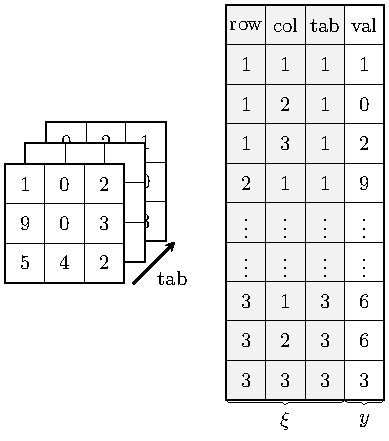
\includegraphics[width=0.2\textwidth]{img/threeway.pdf} &
    \footnotesize (b)
    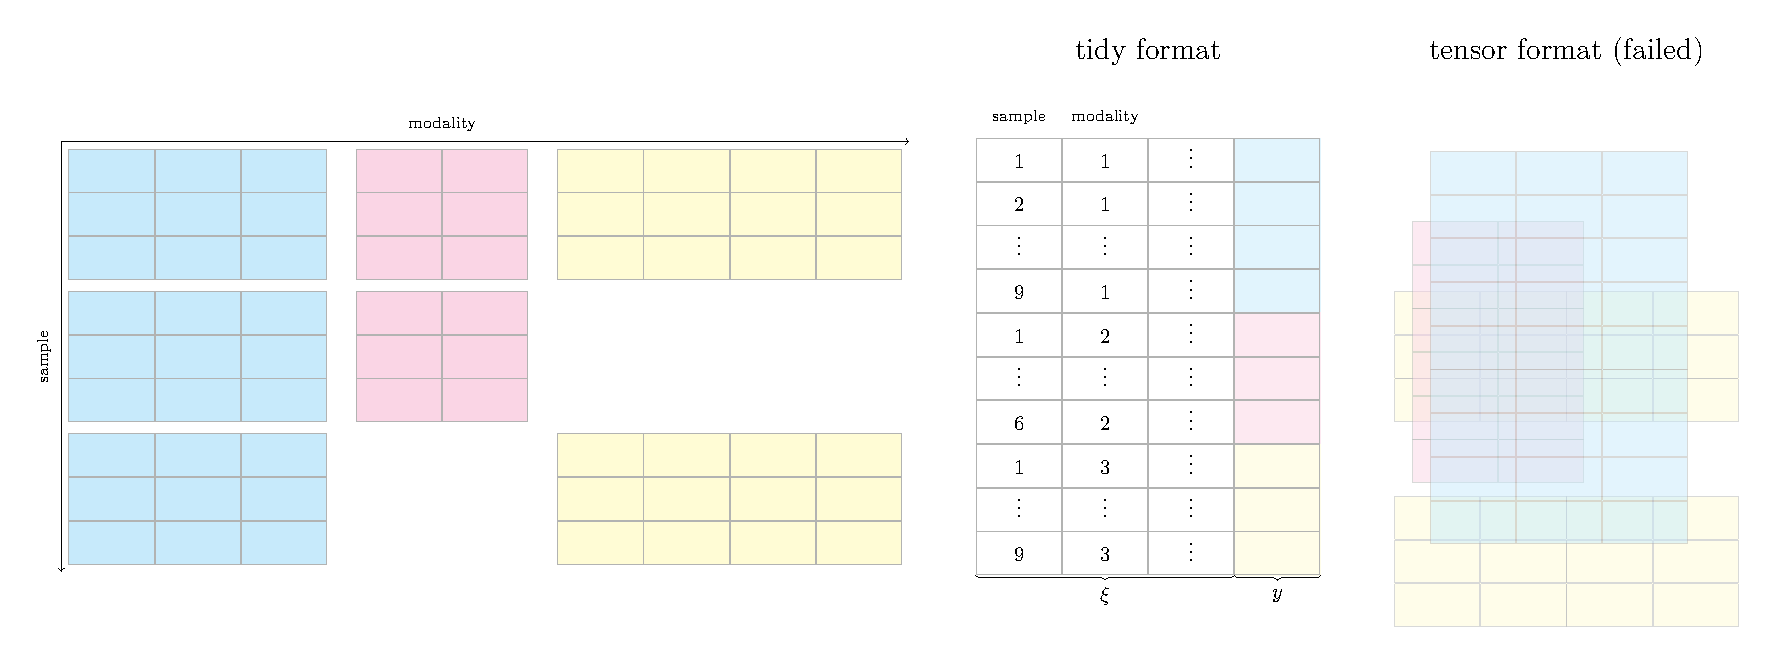
\includegraphics[width=0.7\textwidth]{img/mosaic.pdf} 
    \end{tabular}
    \caption{semi-pared なデータの統合. (a)多次元配列は右に示す形式(tidy-format)でも表現できる.  (b) 多次元配列の形式での対応づけが難しいデータを tidy-formatで保存できる. ここで白いセルは欠測を意味する.}
    \label{fig_mosaic}
\end{figure}

次の節でここまでの議論を確率モデルとして定式化する.

\subsection{モデル}
まずいくつか記号を定める. 大きさ $N$ の組の変数 $(y_n, \xi_n)$, ($n=1,\ldots, N$)が観測されるとする. $\xi_n$ は $y_n$と対応する任意の質的変数のベクトルである. また $y=(y_1, \ldots, y_N)'$, $\Xi=(\xi_1, \ldots \xi_N)'$ とこれらをまとめて表記する.
$\xi_n$ は(例えばワンホットエンコーディングを用いることによって)2値変数のベクトル $x_n$ に写すことができる. この記法の下で, 次のデータ生成過程を考える.
\begin{align}
y_{n} &= A_{m(n)}(z_{n}), \quad (z_{n} \mid V, \lambda) \sim \mathcal{N}\left(z_n \mid \sum_{l=1}^L \prod_{d=1}^Dv_{dl}^{x_{ndm}}, \lambda^{-1}_m\right)  \label{eq_mod1}\\
\lambda & \sim \gam(\lambda | a,b). \nonumber
\end{align}
ここで $V=(v_{dl})$ は $D \times L$  行列であり推定の対象となる潜在変数である. $\gam(x|a,b)$ は形状パラメータとレートパラメータがそれぞれ $a$ と $b$のガンマ分布を表す. また $z_n$, $A_{m}(z)$, $m(n)$ という新しい記号を導入したので順に説明する. これらはモダリティによって $y$ の取りうる値の範囲が明確に変わる場合を考えるためのものである.
例を上げると, データに負の値が生じないことが明らかなとき, $0$ を$1$と予測することと$-1$と予測することは対称に評価できない.
そのため, 分布の台の変化に対応すべく, 次の中間的な変数 $z_n$を考える.
関数 $A_m(x)$ は次のいずれかから分析者が選択する.
\begin{itemize}
\item $y_m$ が実数(連続)値をとるとき: 
$$
A_m(x)=x.
$$
\item $y_m$ が非負のとき:
$$
A_m(x)=\begin{cases}x, &x>0\\0 &x\leq 0\end{cases}.
$$
\item
$y_m$ が2値(0 or 1)のとき:
$$
A_m(x)=\one_{[0,\infty)}(x).
$$
\item
$y_n$ が非負の整数のとき:
$$
A(x)=\begin{cases}\lceil x\rceil, & x>0\\0 &x\leq 0\end{cases}.
$$
\end{itemize}
ここで $\one_{[0,\infty)}(x)$ は指示関数とした.
$m(n)$ は $n$ をモダリティを区別する添字に写す関数とした. これにより複数のモダリティを考慮し, 各モダリティの分布を変更できる.

また $v_{dl}$ の事前分布については, 次のように非負制約の有無によって使い分ける.
\begin{align}
v_{dl} & \sim \normal(v_{dl} | 0,\tau^{-1}), \quad  \mbox{(非負のとき)} \label{eq_prior1}, \\
v_{dl} & \sim \truncnorm(v_{dl} | 0, \tau^{-1}), \quad  \mbox{(負の値を許すとき).} \label{eq_prior2}
\end{align}
ここで $\truncnorm(x | \mu, \sigma^2)$ は0で左側を切断された正規分布である.
この切断正規分布は次のように書ける.
\begin{equation*}
   \truncnorm(x | \mu, \sigma^2) \propto    \normal(x | \mu, \sigma^2) \one_{[0,\infty)}(x) 
\end{equation*}

非負制約の有無は$v_{dl}$ごとに設定できるとしてもこの節の議論に矛盾は生じないが, 我々の実装では指定された1つの変数のみに負の値を許すことにした. これは$1=(-1)\times(-1)$によって解釈が煩雑になるのを避けるためである.

ここまで述べたモデルに基づき $v_{dl}$ についての対数尤度関数 $\ell(v_{dl})$は次のように書ける.
\begin{align*}
& \ell(v_{dl}) =\sum_{n=1}^{N} \log p(z|V, X)\\
&= \sum_{n=1}^{N}\left(-\frac{\lambda}{2}\left\{ z_n -\sum_{l=1}^L\prod_{d=1}^D v_{dl}^{x_{nd}} \right\}^2\right)+ \C\\
&= -\sum_{m=1}^M\frac{h_{dlm}}{2}\left(v_{dl}^2-2v_{dl}\frac{\eta_{dlm}}{h_{dlm}}\right) +C.
\end{align*}
ここでは $v_{dl}$に依存しない項を$C$ とまとめて置き, $\eta_{dl}$ と $h_{dl}$ は次のように置いた.
\begin{align}
\eta_{dl} &= \sum_n x_{nd} \prod_{d' \neq d} v_{dl}^{x_{ndm}}\left( z_{n} - \sum_{l'\neq l} \prod_{d' \neq d} v_{dl}^{x_{nd}} \right) \label{eq_eta}\\
h_{dl} &= \sum_n \lambda x_{n} \prod_{d' \neq d} v_{dl}^{2x_{nd}}. \label{eq_h}
\end{align}
ここから推定のためのアルゴリズムを導くことができる.

\subsection{変分ベイズ法}
\label{est_sec}
この節では変分EMアルゴリズム\cite{Jordan}に基づき, 提案モデルについての推定量を導出する. 
本研究では平均場近似の仮定を置く. すなわち, 近似事後分布が互いに独立とした下でカルバックライブラ情報量の意味で事後分布を近似する$q(v_{dl})$ と $q(\lambda)$ を求める. また変分事後分布による$x$の期待値を $\langle x \rangle$ と表記する.
$v_{dl}$についての変分事後分布として次を得る.
\begin{align}
q(v_{dl})= \begin{cases}
\normal(\mu_{dl}, \sigma_{dl}) & \mbox{when the prior of $v_{dl}$ is not truncated} \\
\truncnorm(\mu_{dl}, \sigma_{dl}) & \mbox{when the prior of $v_{dl}$ is truncated},     
\end{cases} \label{qv}
\end{align}
ここで $\mu_{dl}$ と $\sigma_{dl}$ は次のように置いた.
\begin{align*}
\mu_{dl} &=\frac{\langle \eta_{dl} \rangle}{\langle h_{dl}\rangle+\tau/\langle\lambda\rangle},\\
\sigma^2 &=\left(\tau + \langle h_{dl} \rangle \right)^{-1}.
\end{align*}
$\lambda$ についての変分事後分布として次を得る. 
\begin{align}
    q(\lambda) = \gam \left(N/2 \eta_{dl}, \left(\sum_m h_{dl}+\tau\right)/2\right). \label{qlam}
\end{align}
変分ベイズ法の更新式で必要な各確率変数の期待値は次の通りである.
\begin{align*}
\langle v_{dl}\rangle &=\mu_{dl} + \sigma_{dl} \phi(-\mu_{dl}/\sigma_{dl})/\Phi(-\mu_{dl}/\sigma_{dl}),\\
\langle v_{dl}^2 \rangle&=\mu_{dl}^2 + \sigma_{dl}^2 + \mu_{dl} \sigma_{dl} \phi(-\mu_{dl}/\sigma_{dl})/\Phi(-\mu_{dl}/\sigma_{dl}),\\
\langle \lambda \rangle &= (N \langle \eta_{dl} \rangle ) / \left( \langle h_{dl} \rangle +\tau\right).
\end{align*}
ここで $\phi(x)$ と $\Phi(x)$ をそれぞれ標準正規分布の確率密度関数, 分布関数とした.

潜在変数 $z_n$, についての期待値はMonte-Carlo積分で評価する.すなわち, $z_n$のMonte-Carloサンプルを特に $\tilde z_n$ と書くことにすると, $\tilde z_n$ を次の変分事後分布から疑似乱数でサンプルする. 
\begin{itemize}
\item $y_n$ が実数(連続)値をとるとき: 
\begin{equation}
z_n=y_n \quad \mbox{(with probability 1)}  \label{qz_iden}
\end{equation}
\item $y_n$ が非負のとき:
\begin{align}
q(-z_n) = \begin{cases}
    \mathcal{TN}(-z_n|-f_n, \sigma_n^2) & y_n=0,\\
    z_n = y_n \mbox{~with probability 1} & y_n>0
\end{cases} \label{qz_rect}
\end{align}
\item $y_n$ が2値(0 or 1)のとき:
\begin{align}
q(-z_n) = \begin{cases}
    \mathcal{TN}(-z_n|-f_n, \sigma_n^2) & y_n=0,\\
    \mathcal{TN}(z_n|f_n, \sigma_n^2) & y_n=1
\end{cases}\label{qz_binary}
\end{align}
\item $y_n$ が非負の整数のとき:
\begin{align}
q(-z_n) = \begin{cases}
    \mathcal{TN}(-z_n|-f_n, \sigma_n^2) & y_n=0,\\
    \mathcal{N}(z_n|f_n, \sigma_n^2) \one_{[y_n,y_n+1]}(z_n) \cdot C & y_n > 0
\end{cases}\label{qz_disc}
\end{align}
\end{itemize}

要約すると, 近似事後分布を実現するアルゴリズムは次のようになる:
\begin{itemize}
\item 変分Eステップ: 式\ref{qz_iden}--\ref{qz_disc} を用いて $\tilde{z}_n$ をサンプルする.
\item 変分Mステップ:  式\ref{qv} を用いて$q(v_{dl})$ を, 式\ref{qlam} を用いて$q(\lambda)$を更新する. 
\end{itemize}

当日はこの推定量の性質を評価するシミュレーションと, 実際的なデータ分析事例をあわせて報告する.

\begin{thebibliography}{9}
\bibitem{Heumos} Heumos L, Schaar AC, Lance C, et al. (2023). Best practices for single cell analysis across modalities. {\em Nature Review Genetics}, 24, 550-572.
\bibitem{AbeShimamura} Abe K \& Shimamura T. (2023). UNMF: A unified non-negative matrix factorization for multi-dimensional omics data. {\em Briefings in Bioinformatics.}  24 (5), bbad253.
\bibitem{Wickham2019} Wickham H. (2019).  {\em Advanced R, second edition}. Chapman and Hall/CRC.
\bibitem{Jordan} Jordan~MI, Ghahramani~Z, Jaakkola~TS \& Saul~LK. (1999). An introduction to variational methods for graphical models. {\em Machine learning}, 37(2), 183-233.
\end{thebibliography}
\end{document}  m 